\documentclass[twocolumn, 12pt]{article}
\usepackage[utf8]{inputenc}
\usepackage{amsmath}
\usepackage{marvosym}
\usepackage{textcomp}
\usepackage{geometry}
\usepackage{array}
\usepackage{wrapfig}
\usepackage{multirow}
\usepackage{graphicx}
\usepackage{float}
\usepackage{wrapfig}
\usepackage{caption}

\geometry{a4paper, margin=.75in}



\begin{document}
\small{



\section*{Mechanics of Materials}
\subsection*{Equations}

\begin{equation*}
     \sigma=\frac{ \textbf{P}}{A} \hspace{15pt} \sigma_B=\frac{\textbf{P}_B}{A_B} \hspace{15pt} \delta=\varepsilon L
\end{equation*}


\begin{equation*}
     \delta=\frac{\textbf{P}L}{EA} \hspace{15pt} \delta_T=\alpha\Delta TL
\end{equation*}

\begin{equation*}
    \delta=\sum_{i=1}^{n} \frac{\textbf{N}_iL_i}{E_iA_i} \hspace{15pt} \delta=\int\limits_0^L \frac{\textbf{N}(x)}{EA(x)}dx
\end{equation*}

\begin{equation*}
    \text{Elongation}=\frac{L_1-L_0}{L_0}100\%  
\end{equation*}

\begin{equation*}
    \text{Area} \text{ Reduction}=\frac{A_0-A_1}{A_0}100\%
\end{equation*}

\begin{equation*}
     E=\frac{\sigma}{\varepsilon} \hspace{15pt }\nu=-\frac{\varepsilon'}{\varepsilon} \hspace{15pt} G=\frac{E}{2(1+\nu)}
\end{equation*}

\begin{equation*}
     \tau_{\text{avg}}=\frac{\textbf{V}}{A} \hspace{15pt}  \tau=G\gamma(\text{radians})
\end{equation*}

\begin{equation*}
     \textit{n}=\frac{\text{actual strength} }{\text{required strength}}=\frac{\text{yield stress}}{\text{allowable stress}}
\end{equation*}

\begin{equation*}
    \textbf{P}=\textit{k}\hspace{1pt} \delta  \hspace{15pt} \textit{k}=\frac{\textbf{P}}{\delta}=\frac{1}{f} \hspace{15pt} f=\frac{\delta}{\textbf{P} }=\frac{1}{\textit{k}} 
\end{equation*}

\begin{equation*}
    \varepsilon_T=\alpha\Delta T \hspace{15pt} \delta_T=\alpha\Delta TL \hspace{15pt} \sigma_T=E\alpha\Delta T
\end{equation*}

\begin{equation*}
    \sigma_{\text{max}}=\sigma_x \hspace{15pt} \tau_{\text{max}}=\frac{\sigma_x}{2}
\end{equation*}

\begin{equation*}
    \tau_{\text{single}}=\frac{\textbf{V}}{A_{\text{pin}}} \hspace{15pt} \tau_{\text{double}}=\frac{\textbf{V}}{2A_{\text{pin}}}
\end{equation*}

\begin{equation*}
    \sigma_{B,\text{ single}}=\frac{\textbf{P}}{d_{\text{pin}}t_{\text{bracket}}} \hspace{15pt} \sigma_{B,\text{ double}}= \frac{\textbf{P}}{2d_{\text{pin}}t_{\text{bracket}} }
\end{equation*}

\begin{equation*}
    \sigma_{x1} =\frac{\sigma_x+\sigma_y}{2} + \frac{\sigma_x-\sigma_y}{2} cos2\theta +\tau_{xy}sin2\theta
\end{equation*}
  
\begin{equation*}
    \sigma_{y1} =\frac{\sigma_x+\sigma_y}{2} - \frac{\sigma_x-\sigma_y}{2} cos2\theta -\tau_{xy}sin2\theta
\end{equation*}

\begin{equation*}
    \tau_{x_1y_1} =-\frac{\sigma_x-\sigma_y}{2} sin2\theta +\tau_{xy}cos2\theta
\end{equation*}

\begin{equation*}
    \sigma_{x1}+\sigma_{y1}=\sigma_x+\sigma_y \hspace{15pt} tan(2\theta_p)= \frac{2\tau_{xy}}{\sigma_x-\sigma_y}
\end{equation*}

\begin{equation*}
    \sigma_{1,2} =\frac{\sigma_x+\sigma_y}{2} \pm \sqrt{\left(\frac{\sigma_x-\sigma_y}{2}\right)^2 +\tau_{xy}^2} 
\end{equation*}

\begin{equation*}
    \sigma_{1,2}=\text{center} \pm \text{radius}
\end{equation*}

\begin{equation*}
    \theta_s=\theta_p \pm 45^\circ \hspace{15pt} \sigma_1 \geq \sigma_2 \geq \sigma_3 \hspace{15pt} \theta=\frac{\phi}{L}
\end{equation*}

\begin{equation*}
    R=\sqrt{\left(\frac{\sigma_x-\sigma_y}{2}\right)^2 +\tau_{xy}^2 } \hspace{15pt}  \theta=\frac{d\phi}{dx} \hspace{15pt} k_T=\frac{T}{\phi}
\end{equation*}

\begin{equation*}
    \gamma_{\text{max}} =r\frac{d\phi}{dx}=r\theta  \hspace{10pt} (\gamma \text{ is measured in radians}) 
\end{equation*}

\begin{equation*}
    \gamma_\rho =\frac{\rho}{r}\gamma_{\text{max}} \hspace{15pt} \tau= Gr\theta= \frac{\rho}{r}\tau_{\text{max}}
\end{equation*}

\begin{equation*}
    I_p=\frac{\pi}{32}(d^4_2 -d^4_1) \hspace{15pt} \tau=\frac{16T}{\pi d^3} \hspace{3pt} (\text{solid only})
\end{equation*}

\begin{equation*}
    \tau_{max} =\frac{Tr}{I_p} \hspace{15pt} \tau =\int_0^L\frac{T(x)}{I_p(x)}dx
\end{equation*}

\begin{equation*}
    \phi=\frac{TL}{GI_p} \hspace{15pt}  \phi= \int_0^L \frac{T(x)}{GI_p(x)}dx
\end{equation*}

\begin{equation*}
    \varepsilon_{max} =\frac{\gamma}{2} \hspace{15pt} \gamma = \frac{\tau}{G} \hspace{15pt} G=\frac{E}{2(1+\nu)}
\end{equation*}

\begin{equation*}
     \mid \sigma_C \mid = \mid \sigma_T \mid = \mid \tau_{\text{max}} \mid \hspace{10pt} (\text{in pure shear only}) 
\end{equation*}

\begin{equation*}
    \psi =\Delta\theta \hspace{15pt} \omega =T \psi \hspace{15pt} \omega = 2\pi f
\end{equation*}

\begin{equation*}
    P=\frac{d \omega}{dt}=T \frac{d \psi}{dt} = T \omega
\end{equation*}

\begin{equation*}
    P = 2 \pi f T \hspace{15pt}  P=\frac{2\pi nT}{60}
\end{equation*}

\begin{equation*}
    \text{RPM}: \hspace{2pt} n = 60f \hspace{15pt} H(\text{Hp})=\frac{2\pi nT}{33,000} \hspace{10pt} \left(\text{Hp}=\frac{\text{ft} \cdot \text{lb}}{\text{s}}\right)
\end{equation*}

\begin{equation*}
    T=2fA_m \hspace{15pt} \tau=\frac{T}{2tA_m}  \hspace{15pt} u=\frac{T^2L}{2GJ}
\end{equation*}

\begin{equation*}
    T_1 = T \frac{G_1I_{p1}}{G_1I_{p1} + G_2I_{p2}} \hspace{15pt}  T_2 =T \frac{G_2I_{p2}}{G_2I_{p2}+G_1I_{p1}}
\end{equation*}

\begin{equation*}
    J=\frac{4tA_m^2}{L_m}  \hspace{15pt} \phi =\frac{TL}{GJ} \hspace{15pt} V=\frac{dM}{dx}
\end{equation*}

\begin{equation*}
    \kappa = \frac{1}{\rho} \hspace{15pt} \sigma =-\frac{y}{\rho}=- \kappa y \hspace{15pt} \kappa = \frac{M}{EI}
\end{equation*}

\begin{equation*}
    \delta = \rho (1-cos\theta) \hspace{15pt} sin\theta = \frac{L/2}{\rho} 
\end{equation*}

\begin{equation*}
    \sigma_x = -\frac{Ey}{\rho} = -E \kappa y \hspace{15pt} \sigma_x = -\frac{My}{I} = \frac{M}{S}
\end{equation*}

\begin{equation*}
    \sigma = \frac{P}{A} - \frac{My}{I} \hspace{15pt} \tau = \frac{VQ}{Ib} \hspace{15pt} S=\frac{I}{y}
\end{equation*}

\begin{equation*}
    \sigma = \frac{P}{A}+\frac{Pey}{I} \hspace{15pt} y_0(\text{adjusted NA})=-\frac{1}{Ae}
\end{equation*}

\begin{equation*}
    Q = (\text{Area})(\text{lever arm from NA to centroid})
\end{equation*}

\begin{equation*}
    \tau _{\text{max}}(\text{rect.})  = \frac{3V}{2A} \hspace{15pt} \tau_{\text{max}}(\text{solid}) = \frac{4V}{3A}
\end{equation*}

\begin{equation*}
    \tau_{\text{max}}(\text{hollow}) = \frac{4V}{3A}\left(\frac{(r_1+r_2)^2} {r_1^2 + r_2^2}\right)
\end{equation*}

\begin{equation*}
    V_{\text{web}}(\text{wide flange}) = \frac{bh_1}{3} (2\tau_{\text{max}}+\tau_{\text{min}}) 
\end{equation*}

\begin{equation*}
    I=\sum_{i=1}^N(I_i+A_id_i^2) \hspace{15pt} d_i=d_{cm}-d_{NA}
\end{equation*}

\begin{equation*}
    M=\kappa (E_1I_1+E_2I_2) \hspace{15pt} \Bar{y} = \frac{\Sigma ydA }{\Sigma dA}
\end{equation*}

\begin{equation*}
    \sigma_{x1,y1}=-n\frac{My}{I_T}  \hspace{15pt}f=\frac{VQ}{I}  
\end{equation*}

\begin{equation*}
    \sigma(\text{spherical})=\frac{pr^2}{2r_mt}=\frac{pr}{2t}
\end{equation*}

\begin{equation*}
    \sigma_1(\text{hoop})=\frac{pr}{t} \hspace{15pt} \sigma_2(\text{axial})=\frac{pr}{2t}
\end{equation*}

\begin{equation*}
    \tau_{\text{max}}(\text{in plane})=\frac{pr}{4t} \hspace{15pt} \tau_{\text{\text{max}}}(\text{any plane})=\frac{pr}{2t}
\end{equation*}

\begin{equation*}
    \varepsilon_{1,2} = \frac{\varepsilon_x +\varepsilon_y}{2} \pm \sqrt{ \left(\frac{\varepsilon_x - \varepsilon_y}{2}\right)^2  + \left(\frac{\gamma_{xy}}{2}\right)^2   }
\end{equation*}

\begin{equation*}
    \varepsilon_{x'} = \frac{\varepsilon_x + \varepsilon_y }{2} + \frac{\varepsilon_x -\varepsilon_y}{2}cos(2\theta) + \frac{\gamma_{xy}}{2} sin(2\theta)
\end{equation*}

\begin{equation*}
    \varepsilon_{y'} = \frac{\varepsilon_x + \varepsilon_y }{2} - \frac{\varepsilon_x -\varepsilon_y}{2}cos(2\theta) - \frac{\gamma_{xy}}{2} sin(2\theta)
\end{equation*}

\begin{equation*}
    tan(2\theta_p) = \frac{\gamma_{xy}}{\varepsilon_x - \varepsilon_y} \hspace{15pt} tan(2\theta_s) = -\frac{\varepsilon_x - \varepsilon_y}{\gamma_{xy}}
\end{equation*}

\begin{equation*}
    S_{\text{req}} = \frac{M_{\text{max}}}{\sigma_{\text{allow}}} \hspace{15pt} EI\frac{d^2v}{dx^2} = M(x) \hspace{15pt} F=qs
\end{equation*}

\begin{equation*}
    \sigma_{cr}=\frac{\pi^2E}{\left(\frac{KL}{r}\right)^2} \hspace{15pt} P_{cr} = \frac{\pi^2EI}{(KL)^2} \hspace{15pt} \frac{1}{\rho} = \frac{M}{EI}
\end{equation*}

\subsection*{Column Boundary Conditions}
\begin{itemize}
    \item Pinned-Pinned K=1
    \item Fixed-Fixed K=0.5
    \item Pinned-Fixed K=0.7
    \item Fixed middle, free ends K=2
\end{itemize}



\subsection*{Releases}
\begin{itemize}
    \item Axial release
    \begin{equation*}
        N=0, \hspace{8pt} V,M \neq 0
    \end{equation*}
    
    \item Shear release
    \begin{equation*}
        V=0, \hspace{8pt} N,M \neq 0
    \end{equation*}
    
    \item Moment release
    \begin{equation*}
        M=0, \hspace{8pt} N,V \neq 0
    \end{equation*}
    
    \item Torque release
    \begin{equation*}
        T=0, \hspace{8pt} N,V,M \neq 0
    \end{equation*}
    

\end{itemize}








\begin{figure}[h]
    \centering
    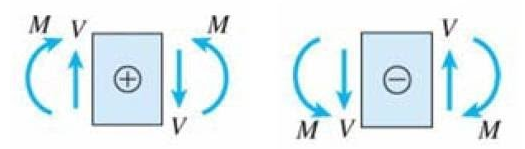
\includegraphics[scale=0.5]{dsc.png}
    \caption*{Deformation sign convention}
    \label{my_label}
\end{figure}

}
\end{document}